\section{Definition of tests} \label{definition_of_tests}

	\subsection{Overview}

		\subsubsection{Importance of Testing}

		Testing plays a critical role in ensuring the functionality, usability, and security of RadiantIQ. As an platform, it must not only meet industry standards for software quality but also provide a reliable and efficient learning experience for our users. Comprehensive testing helps identify and address issues early in the development process, reducing critical issues impacting the user experience post-deployment.

		\subsubsection{Scope}

		This document outlines the testing strategy for RadianIQ, detailing the objectives, testing types, approach, test cases, test environment, test execution process, risks, and mitigation strategies. It serves as a guideline for the testing team, developers, and stakeholders involved in the development and quality assurance of the application.

		\subsubsection{Audience}
		
		The intended audience includes:
		
		\begin{itemize}
			\item Development team: To understand the testing requirements and incorporate them into the development process.
			\item Quality assurance team: To execute the testing procedures outlined in this document and ensure the quality of the application.
			\item Project stakeholders: To gain insights into the testing strategy and its implications on the overall project timeline.
		\end{itemize}
		
		
		
	\subsection{Testing Objectives}
	
		\subsubsection{Goals of the Testing Strategy}
		
		The primary objective is to ensure that the platform meets the highest standards of quality, reliability, and security. Specifically, it aims to:
		
		\begin{itemize}
			\item Verify the functionality of all features: Ensure that each function of the web application, including course and class management, user registration, content delivery, and communication features, works as intended without any errors or unexpected behavior.
			\item Assess usability and accessibility: Evaluate the user-friendliness and accessibility of the platform to ensure that users can navigate the application easily and perform their tasks efficiently.
			\item Ensure compatibility across different environments: Confirm that RadianIQ is compatible with various browsers (e.g., Chrome, Firefox, Safari), devices (e.g., desktops, laptops, tablets, smartphones), and operating systems (e.g., Windows, macOS, iOS, Android).
			\item Evaluate performance: Test the responsiveness and scalability of the application to ensure that it can handle multiple users accessing the platform simultaneously and perform well under high peak.
			\item Identify and mitigate security vulnerabilities: Conduct thorough security testing to identify potential vulnerabilities, such as data breaches, unauthorized access, and injection attacks, and implement measures to mitigate these risks and protect user data.
			\item Ensure integration between components: Validate the interaction between different components and modules of the platform to ensure seamless functionality and data exchange.
		\end{itemize}

		
	\subsection{Testing Types}
		
		\subsubsection{Functional Testing (Black-box Testing)}
		
		Functional testing ensures that each function of RadianIQ works as expected. This involves testing individual features and functionalities to verify that they meet the specified requirements, including:
		
		\begin{itemize}
			\item Course Management: Testing the creation, editing, and deletion of courses, including features such as adding course materials, setting up assessments, and managing enrollments.
			\item Class Management: Testing the creation, editing, and deletion of classes, including features such as creating class sessions, managing student registrations, tracking student progress, and grading assignments.
			\item User Registration and Authentication: Testing the registration process for all the user roles, as well as the login and authentication mechanisms to ensure secure access to the platform.
			\item Content Delivery: Testing the delivery of course content, including multimedia materials, documents, mini games, and lectures, to ensure they are accessible and functional.
			\item Communication Features: Testing messaging systems, discussion forums, and collaboration tools to ensure smooth communication and interaction between users.
		\end{itemize}

		\subsubsection{Structural Testing (White-box Testing)}

		Structural testing, or white-box testing, involves examining the internal structure and code of the e-learning web application to validate its logic, algorithms, and internal pathways. This testing type ensures the reliability, security, and maintainability of the application's underlying codebase. Key aspects to test include:

		\begin{itemize}
			\item Code Coverage: Verify that all code paths, including branches, loops, and conditionals, are executed and tested to achieve high code coverage.
			\item Data Validation: Validate input data to prevent security vulnerabilities such as SQL injection, cross-site scripting (XSS), and data manipulation attacks.
			\item Error Handling: Ensure robust error handling mechanisms are in place to gracefully handle exceptions, invalid inputs, and unexpected scenarios without crashing the application.
			\item Performance Optimization: Analyze code performance to identify and optimize inefficient algorithms, database queries, and resource-intensive operations for improved scalability and responsiveness.
		\end{itemize}
		
		\subsubsection{Usability Testing}
		
		Usability testing focuses on assessing the user-friendliness and accessibility of the platform. This involves evaluating the interface design, navigation flow, and overall user experience to ensure that users can easily accomplish their tasks and achieve their learning objectives. Usability testing includes:
		
		\begin{itemize}
			\item Navigation Testing: Evaluating the navigation flow within the application to ensure that users can easily find and access the desired features and content.
			\item Accessibility Testing: Ensuring that the platform is accessible to users with disabilities, including compliance with accessibility standards such as WCAG (Web Content Accessibility Guidelines).
			\item User Feedback Analysis: Gathering feedback from users through surveys, interviews, or usability testing sessions to identify areas for improvement in the user interface and experience.
		\end{itemize}
		
		\subsubsection{Compatibility Testing}
		
		Compatibility testing ensures that RadianIQ is compatible across different browsers, devices, and operating systems. This involves testing the application on various combinations of browsers (e.g., Chrome, Firefox, Safari), devices (e.g., desktops, laptops, tablets, smartphones), and operating systems (e.g., Windows, macOS, iOS, Android) to ensure consistent performance and functionality.
		
		\subsubsection{Performance Testing}
		
		Performance testing evaluates the responsiveness and scalability of the platform under various loads. This involves testing the application's performance metrics such as response time, throughput, and resource utilization to ensure optimal performance under normal and peak usage conditions. Performance testing includes:
		
		\begin{itemize}
			\item Load Testing: Simulating multiple users accessing the platform simultaneously to assess its response time and behavior under heavy loads.
			\item Stress Testing: Pushing the system beyond its normal capacity to identify its breaking point and evaluate its ability to recover under stress.
			\item Scalability Testing: Testing the application's ability to scale resources dynamically to accommodate increasing user loads without degradation in performance.
		\end{itemize}
		
		\subsubsection{Security Testing}
		
		Security testing aims to identify and mitigate potential security vulnerabilities in the platform. This involves testing the application for vulnerabilities such as data breaches, unauthorized access, injection attacks, and XSS (cross-site scripting) attacks. Security testing includes:
		
		\begin{itemize}
			\item Vulnerability Assessment: Identifying potential security vulnerabilities through automated scanning tools and manual code reviews.
			\item Penetration Testing: Simulating real-world attacks to exploit vulnerabilities and assess the effectiveness of security controls and countermeasures.
			\item Data Protection Testing: Ensuring that sensitive user data such as personal information, grades, and assessment results are securely stored, transmitted, and accessed according to privacy regulations and best practices.
		\end{itemize}

		
	\subsection{Testing Approach}

		\subsubsection{V-Model Testing}

		\begin{figure}[H]
			\centering
			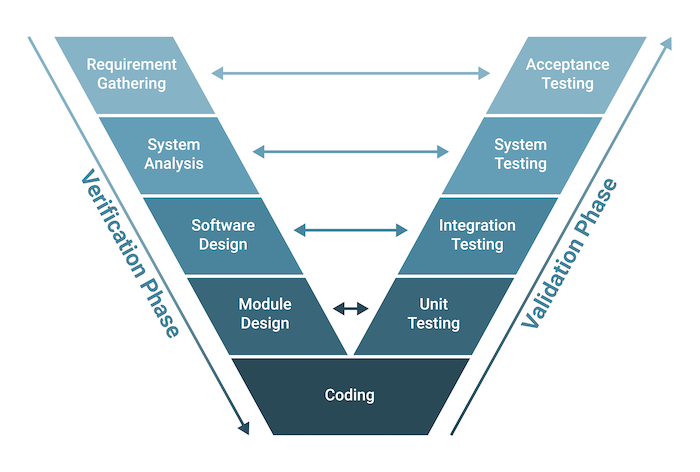
\includegraphics[width=0.55\linewidth]{images/v-model-testing.png}
			\caption{V-model testing}
			\label{fig:v-model-testing}
		\end{figure}

		The V-Model testing approach aligns testing activities with corresponding development phases, emphasizing the relationship between requirements, design, implementation, and testing. In the V-Model, each phase of the development lifecycle has a corresponding testing phase, ensuring comprehensive validation at each stage. The V-Model testing process includes:

		\begin{itemize}
			\item Acceptance Testing (Requirements Gathering): During the requirements gathering phase, acceptance testing focuses on validating the gathered requirements to ensure they are clear, complete, and consistent. This involves collaborating with stakeholders to define acceptance criteria and validate that the requirements accurately capture the needs of end-users and align with business objectives.
			\item System Testing (System Analysis): In the system analysis phase, system testing verifies the complete integrated system against the specified requirements and design specifications. This includes testing the system as a whole to ensure that all components function correctly together and meet the intended functionality, performance, and usability criteria.
			\item Integration Testing (Software Design): Integration testing validates the interaction and integration between individual software modules or components. It ensures that modules interact correctly, exchange data seamlessly, and function as expected within the larger system architecture. Integration testing verifies that the software design, including interfaces and dependencies, is implemented correctly and that modules work together harmoniously.
			modules.
			\item Unit Testing (Module Design): Unit testing focuses on validating the functionality of individual software modules or components in isolation. It verifies that each module performs its intended function according to the specified design and requirements. Unit tests are designed to test specific inputs, outputs, and internal logic of modules, ensuring that each unit operates correctly and meets its design specifications.
		\end{itemize}

		\subsubsection{Manual Testing}
		
		Manual testing involves human testers executing test cases and evaluating the application's behavior based on predefined criteria. This approach allows testers to identify visual inconsistencies, usability issues, and other aspects that may be challenging to automate. The manual testing process includes:
		
		\begin{itemize}
			\item Test Case Creation: Developing detailed test cases based on functional requirements and user stories.
			\item Test Execution: Performing manual tests according to the test cases, documenting observations, and verifying expected outcomes.
			\item Exploratory Testing: Conducting ad-hoc testing to explore the application and uncover potential issues that may not be covered by predefined test cases.
			\item Usability Testing: Engaging real users to evaluate the application's usability, accessibility, and overall user experience.
			\item Regression Testing: Repeating tests to ensure that new features or changes do not adversely affect existing functionalities.
		\end{itemize}
		
		\subsubsection{Automated Testing}
		
		Automated testing involves using software tools and frameworks to automate the execution of test cases, thereby increasing efficiency, repeatability, and coverage. This approach is particularly useful for repetitive tasks and regression testing. The automated testing process includes:
		
		\begin{itemize}
			\item Test Script Development: Writing test scripts using automated testing tools such as Selenium, Cypress, or TestComplete to simulate user interactions and verify expected behaviors.
			\item Test Suite Creation: Organizing test scripts into test suites based on functional areas or features for efficient execution and maintenance.
			\item Continuous Integration (CI) Integration: Integrating automated tests into the CI/CD pipeline to automatically trigger tests upon code changes and provide rapid feedback to developers.
			\item Cross-Browser and Cross-Platform Testing: Executing tests across different browsers, devices, and operating systems to ensure compatibility and consistent behavior.
			\item Performance Testing Automation: Utilizing tools like JMeter or Gatling for automating performance tests to simulate various load scenarios and analyze system performance metrics.
		\end{itemize}
		
		\subsubsection{Regression Testing}
		
		Regression testing ensures that new changes or enhancements do not introduce unintended side effects or break existing functionalities. The regression testing process includes:
		
		\begin{itemize}
			\item Test Case Maintenance: Updating existing test cases and creating new ones to accommodate changes in the application.
			\item Test Suite Prioritization: Prioritizing test cases based on their criticality and impact on the application to optimize testing efforts.
			\item Automated Regression Testing: Automating repetitive regression tests to ensure consistent and efficient validation of core functionalities.
			\item Manual Regression Testing: Performing manual regression tests for areas that are difficult to automate or require human judgment.
			\item Version Control Integration: Integrating regression tests with version control systems to track changes and ensure test coverage across different software versions.
		\end{itemize}
		
		\subsubsection{Exploratory Testing}
		
		Exploratory testing is a hands-on approach to testing that emphasizes learning, discovery, and experimentation. Testers explore the application with minimal predefined scripts, allowing them to uncover unforeseen issues and gain insights into the user experience. The exploratory testing process includes:
		
		\begin{itemize}
			\item Session-Based Testing: Setting specific time-boxed sessions to focus on exploring different areas of the application.
			\item Bug Reporting: Documenting any issues encountered during exploratory testing, including steps to reproduce and screenshots.
			\item Collaborative Testing: Encouraging collaboration between testers to share insights, findings, and test ideas during exploratory sessions.
			\item Feedback Loop: Providing feedback to developers and stakeholders based on the discoveries made during exploratory testing to drive improvements in the application.
		\end{itemize}
		
		\subsubsection{User Acceptance Testing (UAT)}
		
		UAT involves validating the platform against user requirements and expectations. It ensures that the application meets the needs of end-users and aligns with business objectives. The UAT process includes:
		
		\begin{itemize}
			\item Test Planning: Collaborating with stakeholders to define UAT scope, objectives, and acceptance criteria.
			\item Test Case Preparation: Developing UAT test cases based on user stories, use cases, and business requirements.
			\item End-User Involvement: Engaging end-users, including students, professors, and administrators, to participate in UAT activities and provide feedback.
			\item Feedback Collection: Gathering feedback from end-users regarding usability, functionality, and overall satisfaction with the application.
			\item Bug Triaging: Prioritizing and addressing issues identified during UAT, collaborate with development teams to implement necessary changes.
		\end{itemize}
		
		
	\subsection{Test Cases}

	To be defined at every sprint.
	
	\subsection{Test Environment}
	
		\subsubsection{Hardware Specifications}
		
		The test environment setup for RadianIQ should include hardware specifications that closely resemble the production environment to ensure accurate testing results. The hardware specifications may include:
		
		\begin{itemize}
			\item Server Configuration: Specifications for the server hosting the web application, including CPU, RAM, and storage capacity.
			\item Client Devices: Specifications for client devices used to access the application, such as desktop computers, laptops, tablets, and smartphones.
			\item Networking Equipment: Details of networking hardware such as routers, switches, and firewalls that may impact network performance and connectivity.
		\end{itemize}
		
		\subsubsection{Software Dependencies}
		
		The test environment should replicate the software dependencies of the production environment to ensure compatibility and accurate testing. This includes:
		
		\begin{itemize}
			\item Operating Systems: Versions of operating systems supported by the platform.
			\item Web Browsers: Versions of web browsers supported by the application, including Chrome, Firefox, Safari, and Edge.
			\item Database Systems: Versions of database management systems (DBMS) used by the application. In this case, MongoDB.
			\item Server Software: Versions of web servers, application servers, and other server software required to run the application.
		\end{itemize}
		
		\subsubsection{Network Configurations}
		
		Network configurations play a crucial role in testing the performance and reliability. The test environment should simulate real-world network conditions to evaluate the application's behavior under different scenarios. This includes:
		
		\begin{itemize}
			\item Internet Connectivity: Ensure stable internet connectivity with sufficient bandwidth to support concurrent user interactions.
			\item Firewall and Security Settings: Configure network security settings to simulate firewall rules and security protocols that may impact application access and communication.
			\item Load Balancing: Implement load balancing configurations to distribute traffic across multiple servers and assess scalability and performance under heavy loads.
			\item Latency and Packet Loss: Introduce latency and packet loss to simulate network congestion and assess application responsiveness and resilience.
		\end{itemize}
		
		\subsubsection{Data Sets for Testing}
		
		Data sets used for testing should represent realistic scenarios and volumes to validate the performance, scalability, and reliability of the platform. This includes:
		
		\begin{itemize}
			\item Sample Courses and Content: Populate the test environment with a variety of sample courses, lectures, mini games, and multimedia content to simulate real usage scenarios.
			\item User Data: Create test user accounts with different roles and varying levels of access permissions to test user registration, authentication, and authorization functionalities.
			\item Test Data Generation: Use data generation tools or scripts to create large volumes of test data to simulate realistic user interactions, such as enrollment in courses, participation in discussions, and submission of assignments.
		\end{itemize}
		
		
	\subsection{Test Execution}
	
		\subsubsection{Test Scheduling}
		
		Test scheduling involves planning and organizing the execution of test cases to ensure efficient use of resources and timely validation of RadianIQ. The test scheduling process includes:
		
		\begin{itemize}
			\item Test Planning: Develop a comprehensive test plan that outlines the testing scope, objectives, test cases, and timelines.
			\item Test Prioritization: Prioritize test cases based on their criticality, impact on the application, and dependencies to focus testing efforts on high-risk areas and critical functionalities.
			\item Test Coverage: Ensure adequate test coverage by scheduling tests to validate all aspects of the application, including core functionalities, user interactions, and edge cases.
			\item Test Execution Schedule: Define a schedule for executing test cases, considering factors such as team availability, testing environment availability, and project milestones.
			\item Iterative Testing: Plan for iterative testing cycles to incorporate feedback, address defects, and validate fixes throughout the software development lifecycle.
		\end{itemize}
		
		\subsubsection{Bug Reporting and Tracking}
		
		Bug reporting and tracking are essential aspects of the test execution process, enabling testers to document and manage issues effectively. The bug reporting and tracking process includes:
		
		\begin{itemize}
			\item Defect Identification: Identify and document defects discovered during test execution, including detailed descriptions, steps to reproduce, and screenshots or logs.
			\item Defect Prioritization: Prioritize defects based on severity, impact on functionality, and business priority to focus on resolving critical issues first.
			\item Defect Management: Assign, track, and manage defects using a centralized defect tracking system or bug management tool to ensure transparency, accountability, and traceability throughout the defect lifecycle.
			\item Defect Resolution: Collaborate with development teams to investigate, triage, and resolve reported defects promptly, following established workflows and communication channels.
		\end{itemize}

		